\chapter{Complessità computazionale}

\index{complessità computazionale}

Nella gare di programmazione l'efficienza di un algoritmo è importante
Mentre è relativamente semplice inventare un algoritmo lento che risolve un problema,
la vera sfida è di inventarne uno veloce.
Se l'algoritmo è tropo lento, prenderà solo parte del punteggio
o addirittura non prenderà nulla.

La \key{complessità computazionale} di un algoritmo
stima quanto tempo impiegherà un algoritmo per trovare la 
soluzione rispetto a un qualche input.
L'idea è quella di rappresentare l'efficienza di un algoritmo
tramite un funzione il cui parametro è la dimensione dell'input.
Calcolando la sua complessità è possibile 
scoprire se un algoritmo sarà veloce abbastanza 
senza doverlo realmente implementare.

\section{Regole per il calcolo della complessità}

Il comportamento asintotico di un algoritmo,
che ne approssima la complessità computazionale,
è indicato con $O(\cdots)$,
dove al posto dei tre punti è presente una funzione.
Normalmente la variabile $n$ indica la dimensione dell'input.
Per esempio, se l'input fosse un array di numeri,
$n$ sarebbe la dimensione dell'array, se invece l'input
fosse una stringa, $n$ sarebbe la lunghezza della stringa. 

\subsubsection*{Cicli}

Solitamente un algoritmo è lento perchè 
contiene molti cicli annidati attraverso cui deve passare l'input.
Più cicli annidati contiene, più risulterà lento.
Se sono presenti $k$ cicli annidati,
la complessità sarà di tipo $O(n^k)$.

Per esempio, la complessità del seguente codice è di tipo $O(n)$:
\begin{lstlisting}
for (int i = 1; i <= n; i++) {
    // codice
}
\end{lstlisting}

mentre invece la complessità di questo codice è di tipo $O(n^2)$:
\begin{lstlisting}
for (int i = 1; i <= n; i++) {
    for (int j = 1; j <= n; j++) {
        // codice
    }
}
\end{lstlisting}

\subsubsection*{Ordine di grandezza}

La complessità non da una misura esatta del numero
di volte che una certa parte di codice è eseguita all'interno di un ciclo,
ma ne mostra solo l'ordine di grandezza.
Negli esempi che seguono, il codice interno ai cicli
è eseguito $3n$, $n+5$ e $\lceil n/2 \rceil$ volte,
ma in ogni caso la complessità è di tipo $O(n)$.

\begin{lstlisting}
for (int i = 1; i <= 3*n; i++) {
    // codice
}
\end{lstlisting}

\begin{lstlisting}
for (int i = 1; i <= n+5; i++) {
    // codice
}
\end{lstlisting}

\begin{lstlisting}
for (int i = 1; i <= n; i += 2) {
    // codice
}
\end{lstlisting}

In questo altro esempio la complessità è di tipo $O(n^2)$:

\begin{lstlisting}
for (int i = 1; i <= n; i++) {
    for (int j = i+1; j <= n; j++) {
        // codice
    }
}
\end{lstlisting}

\subsubsection*{Fasi}

Se un algoritmo è formato da una serie di fasi una dopo l'altra,
la complessità computazione è la più grande 
tra le complessità di ogni singola fase.
Il motivo è che
la fase più lenta risulta il collo di bottiglia del programma.

Per esempio, nel codice seguente sono presenti
tre fasi con complessità
$O(n)$, $O(n^2)$ and $O(n)$, quindi la complessità totale è di tipo $O(n^2)$.

\begin{lstlisting}
for (int i = 1; i <= n; i++) {
    // codice
}
for (int i = 1; i <= n; i++) {
    for (int j = 1; j <= n; j++) {
        // codice
    }
}
for (int i = 1; i <= n; i++) {
    // codice
}
\end{lstlisting}

\subsubsection*{Variabili multiple}

A volte la complessità dipende da più fattori.
Se questo è il caso, la formula della complessità può contenere 
diverse variabili.

Per esempio, la complessità del seguente codice è $O(nm)$:

\begin{lstlisting}
for (int i = 1; i <= n; i++) {
    for (int j = 1; j <= m; j++) {
        // codice
    }
}
\end{lstlisting}

\subsubsection*{Ricorsione}

La complessità di una funzione ricorsiva dipende
dal numero di volte che una funzione viene chiamata
e dalla complessità di ogni singola chiamata.
La complessità totale è il prodotto di questi valori.

Per esempio, si consideri la seguente funzione:

\begin{lstlisting}
void f(int n) {
    if (n == 1) return;
    f(n-1);
}
\end{lstlisting}
La chiamata $\texttt{f}(n)$ produce $n$ chiamate ricorsive,
e la complessità di ogni chiamata è $O(1)$, quindi la complessità totale è $O(n)$.

Si consideri quest'altra funzione: 

\begin{lstlisting}
void g(int n) {
    if (n == 1) return;
    g(n-1);
    g(n-1);
}
\end{lstlisting}
In questo caso ogni funzione genera due chiamate ricorsive, tranne
l'ultima per $n=1$.
Si osservi nella tabella cosa succede quando $g$ è chiamata con
il parametro $n$, attraverso "l'esplosione" di tutte le chiamate:
\begin{center}
\begin{tabular}{rr}
chiamata & numero di chiamate \\
\hline
$g(n)$ & 1 \\
$g(n-1)$ & 2 \\
$g(n-2)$ & 4 \\
$\cdots$ & $\cdots$ \\
$g(1)$ & $2^{n-1}$ \\
\end{tabular}
\end{center}
Come si può vedere, la complessità risulta quindi
\[1+2+4+\cdots+2^{n-1} = 2^n-1 = O(2^n).\]

\section{Classi di complessità computazionale}

\index{classi di complessità}

Nella seguente lista si possono trovare le classi di
complessità computazionale più comuni

\begin{description}
\item[$O(1)$]
\index{Complessità costante}
Il tempo di esecuzione di un algoritmo con complessità \key{costante}
non dipende dalla dimensione dell'input.
Un tipico esempio è una formula che calcola
direttamente la risposta.

\item[$O(\log n)$]
\index{Complessità logaritmica}
Un algoritmo con complessità \key{logaritmica} spesso divide
l'input in due parti uguali a ogni passaggio.
Il tempo di esecuzione è quindi logaritmico, perchè 
$\log_2 n$ è il numero di volte che $n$ deve
essere diviso per 2 per ottenere 1.

\item[$O(\sqrt n)$]
Un algoritmo con complessità di tipo \key{radice quadrata} è più lento di 
$O(\log n)$ ma più veloce che $O(n)$.
Una proprietà della radice quadrata è che
$\sqrt n = n/\sqrt n$, il che vuol dire, in un certo senso,
che $\sqrt n$ si trova nel mezzo dell'input.

\item[$O(n)$]
\index{complessità lineare}
Un algoritmo di tipo \key{lineare} attraversa l'input 
un numero di volte che dipende direttamente dalla dimensione dell'input.
In molti algoritmi questa è la migliore complessità possibile,
poichè spesso è necessario accedere ad ogni elemento in input 
prima di poter dare la risposta.

\item[$O(n \log n)$]
Questa complessità molte volte indica che l'algoritmo
deve ordinare l'input,
poichè la complessità di un algoritmo di ordinamento efficiente è di tipo
$O(n \log n)$.
Un'altra possibilità è che l'algoritmo utilizzi una struttura dati
dove ogni operazione richiede un costo $O(\log n)$.

\item[$O(n^2)$]
\index{complessità quadratica}
Un algoritmo \key{quadratico} spesso richiede 
due cicli annidati e quindi comporta che 
il passaggio attraverso tutte le possibili coppie di 
indici richieda un costo di tipo $O(n^2)$.

\item[$O(n^3)$]
\index{complessità cubica}
Un algoritmo di tipo cubico spesso contiene tre cicli 
annidati e quindi comporta che 
il passaggio attraverso tutte le possibili triplette di 
indici richieda un costo di tipo $O(n^3)$.

\item[$O(2^n)$]
Questa complessità indica spesso che l'algoritmo 
abbia necessità di iterare attraverso tutti i sottoinsiemi 
degli elementi in input.
Per esempio, i sottoinsiemi di $\{1,2,3\}$ sono
$\emptyset$, $\{1\}$, $\{2\}$, $\{3\}$, $\{1,2\}$,
$\{1,3\}$, $\{2,3\}$ e $\{1,2,3\}$.

\item[$O(n!)$]
Questa complessità spesso indica che l'algoritmo 
abbia la necessità di iterare attraverso tutte
le permutazioni degli elementi in input.

Per esempio, le permutazioni di $\{1,2,3\}$ sono
$(1,2,3)$, $(1,3,2)$, $(2,1,3)$, $(2,3,1)$,
$(3,1,2)$ e $(3,2,1)$.

\end{description}

\index{algoritmi polinomiali}
Un algoritmo è \key{polinomiale}
se la sua complessità è al massimo di tipo $O(n^k)$
dove $k$ è una costante.
Tutte le complessità viste in precedenza eccetto
$O(2^n)$ e $O(n!)$ sono polinomiali.
Spesso nella pratica la costante $k$ è piccola.
e quindi la complessità polinomiale
può comunque essere considerata efficiente.

\index{Problemi NP-hard}

La maggior parte degli algoritmi in questo libro
sono di tipo polinomiale.
Comunque ci sono molti problemi importanti per cui
non si conosce un algoritmo risolutivo di tipo polinomiale,
cioè nessuno sa come risolverli in maniera efficiente.
I problemi \key{NP-hard} sono un'importante classe di problemi, 
per i quali non è conosciuto nessun algoritmo 
risolutivo di tipo polinomiale\footnote{Un classico libro su questo argomento è
M. R. Garey's e D. S. Johnson's
\emph{Computers and Intractability: A Guide to the Theory
of NP-Completeness} \cite{gar79}.}.

\section{Stimare l'efficienza}

Calcolare la complessità computazionale di un algoritmo
permette di stimare se è possibile arrivare a una soluzione efficiente
del problema senza dover effettivamente implementare l'algoritmo.

Il punto di partenza della stima risiede nel fatto che 
un computer moderno è in grado di svolgere centinaia di 
milioni di operazioni ogni secondo.

Per esempio, si assuma che il tempo limite per un dato
problema sia di 1 secondo e che la dimensione dell'input sia $n=10^5$.
Se la complessità fosse di tipo $O(n^2)$,
l'algoritmo effettuerebbe all'incirca $(10^5)^2=10^{10}$ operazioni.
Questo porterebbe a un tempo di esecuzione di almeno qualche decina di secondi,
così un algoritmo di tipo quadratico sarebbe troppo lento per 
risolvere il problema.

D'altro canto, data la dimensione dell'input,
è possibile \emph{ipotizzare} quale sia la complessità
richiesta a un algoritmo che possa risolvere il problema
soddisfacendo i vincoli temporali richiesti.
Nella tabella seguente si possono trovare alcune stime 
dato un tempo limite di esecuzione di 1 secondo.

\begin{center}
\begin{tabular}{ll}
Dimensione dell'input & Complessità richiesta \\
\hline
$n \le 10$ & $O(n!)$ \\
$n \le 20$ & $O(2^n)$ \\
$n \le 500$ & $O(n^3)$ \\
$n \le 5000$ & $O(n^2)$ \\
$n \le 10^6$ & $O(n \log n)$ o $O(n)$ \\
$n$ molto grande & $O(1)$ o $O(\log n)$ \\
\end{tabular}
\end{center}

Per esempio, se la dimensione dell'input fosse $n=10^5$,
è probabile che la complessità dell'algoritmo necessario
per risolverlo sia di tipo $O(n)$ o $O(n \log n)$.
Questa informazione semplifica la progettazione dell'algoritmo,
poichè elimina tutti gli ipotetici algoritmi 
con complessità maggiore.

\index{fattore costante}

Va comunque ricordato che la complessità è solo una
stima dell'efficienza di un algoritmo,
perchè non tiene conto dei \emph{fattori costanti}.
Per esempio, un algoritmo che ha una complessità di tipo $O(n)$,
può eseguire sia $n/2$ che $5n$ operazioni e 
questo ovviamente può cambiare radicalmente il tempo
di esecuzione di un algoritmo.

\section{Maximum subarray sum}

\index{maximum subarray sum}

There are often several possible algorithms
for solving a problem such that their
time complexities are different.
This section discusses a classic problem that
has a straightforward $O(n^3)$ solution.
However, by designing a better algorithm, it
is possible to solve the problem in $O(n^2)$
time and even in $O(n)$ time.

Given an array of $n$ numbers,
our task is to calculate the
\key{maximum subarray sum}, i.e.,
the largest possible sum of 
a sequence of consecutive values
in the array\footnote{J. Bentley's
book \emph{Programming Pearls} \cite{ben86} made the problem popular.}.
The problem is interesting when there may be
negative values in the array.
For example, in the array
\begin{center}
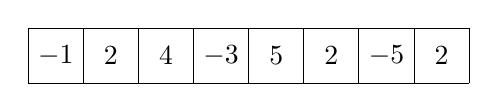
\begin{tikzpicture}[scale=0.7]
\draw (0,0) grid (8,1);

\node at (0.5,0.5) {$-1$};
\node at (1.5,0.5) {$2$};
\node at (2.5,0.5) {$4$};
\node at (3.5,0.5) {$-3$};
\node at (4.5,0.5) {$5$};
\node at (5.5,0.5) {$2$};
\node at (6.5,0.5) {$-5$};
\node at (7.5,0.5) {$2$};
\end{tikzpicture}
\end{center}
\begin{samepage}
the following subarray produces the maximum sum $10$:
\begin{center}
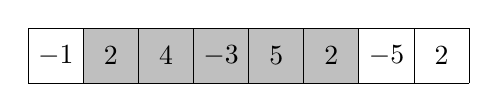
\begin{tikzpicture}[scale=0.7]
\fill[color=lightgray] (1,0) rectangle (6,1);
\draw (0,0) grid (8,1);

\node at (0.5,0.5) {$-1$};
\node at (1.5,0.5) {$2$};
\node at (2.5,0.5) {$4$};
\node at (3.5,0.5) {$-3$};
\node at (4.5,0.5) {$5$};
\node at (5.5,0.5) {$2$};
\node at (6.5,0.5) {$-5$};
\node at (7.5,0.5) {$2$};
\end{tikzpicture}
\end{center}
\end{samepage}

\subsubsection{Algorithm 1}

A straightforward way to solve the problem
is to go through all possible subarrays,
calculate the sum of values in each subarray and maintain
the maximum sum.
The following code implements this algorithm:

\begin{lstlisting}
int best = 0;
for (int a = 0; a < n; a++) {
    for (int b = a; b < n; b++) {
        int sum = 0;
        for (int k = a; k <= b; k++) {
            sum += array[k];
        }
        best = max(best,sum);
    }
}
cout << best << "\n";
\end{lstlisting}

The variables \texttt{a} and \texttt{b} fix the first and
last index of the subarray,
and the sum of values is calculated to the variable \texttt{sum}.
The variable \texttt{best} contains the maximum sum found during the search.

The time complexity of the algorithm is $O(n^3)$,
because it consists of three nested loops 
that go through the input.

\subsubsection{Algorithm 2}

It is easy to make Algorithm 1 more efficient
by removing one loop from it.
This is possible by calculating the sum at the same
time when the right end of the subarray moves.
The result is the following code:

\begin{lstlisting}
int best = 0;
for (int a = 0; a < n; a++) {
    int sum = 0;
    for (int b = a; b < n; b++) {
        sum += array[b];
        best = max(best,sum);
    }
}
cout << best << "\n";
\end{lstlisting}
After this change, the time complexity is $O(n^2)$.

\subsubsection{Algorithm 3}

Surprisingly, it is possible to solve the problem
in $O(n)$ time\footnote{In \cite{ben86}, this linear-time algorithm
is attributed to J. B. Kadane, and the algorithm is sometimes
called \index{Kadane's algorithm} \key{Kadane's algorithm}.}, which means
that just one loop is enough.
The idea is to calculate, for each array position,
the maximum sum of a subarray that ends at that position.
After this, the answer for the problem is the
maximum of those sums.

Consider the subproblem of finding the maximum-sum subarray
that ends at position $k$.
There are two possibilities:
\begin{enumerate}
\item The subarray only contains the element at position $k$.
\item The subarray consists of a subarray that ends
at position $k-1$, followed by the element at position $k$.
\end{enumerate}

In the latter case, since we want to
find a subarray with maximum sum,
the subarray that ends at position $k-1$
should also have the maximum sum.
Thus, we can solve the problem efficiently
by calculating the maximum subarray sum
for each ending position from left to right.

The following code implements the algorithm:
\begin{lstlisting}
int best = 0, sum = 0;
for (int k = 0; k < n; k++) {
    sum = max(array[k],sum+array[k]);
    best = max(best,sum);
}
cout << best << "\n";
\end{lstlisting}

The algorithm only contains one loop
that goes through the input,
so the time complexity is $O(n)$.
This is also the best possible time complexity,
because any algorithm for the problem
has to examine all array elements at least once.

\subsubsection{Efficiency comparison}

It is interesting to study how efficient 
algorithms are in practice.
The following table shows the running times
of the above algorithms for different
values of $n$ on a modern computer.

In each test, the input was generated randomly.
The time needed for reading the input was not
measured.

\begin{center}
\begin{tabular}{rrrr}
array size $n$ & Algorithm 1 & Algorithm 2 & Algorithm 3 \\
\hline
$10^2$ & $0.0$ s & $0.0$ s & $0.0$ s \\
$10^3$ & $0.1$ s & $0.0$ s & $0.0$ s \\
$10^4$ & > $10.0$ s & $0.1$ s & $0.0$ s \\
$10^5$ & > $10.0$ s & $5.3$ s & $0.0$ s \\
$10^6$ & > $10.0$ s & > $10.0$ s & $0.0$ s \\
$10^7$ & > $10.0$ s & > $10.0$ s & $0.0$ s \\
\end{tabular}
\end{center}

The comparison shows that all algorithms
are efficient when the input size is small,
but larger inputs bring out remarkable
differences in the running times of the algorithms.
Algorithm 1 becomes slow
when $n=10^4$, and Algorithm 2
becomes slow when $n=10^5$.
Only Algorithm 3 is able to process
even the largest inputs instantly.
